% 图:eBPF 流水线。视觉词汇:工件=白框,执行组件=蓝色填充框,动作=箭头标签(distribute、load);
% 目标机器内部虚线横隔线分 user space 与 kernel 两带,带标签在框外左侧,证明图例填入 user space 带右侧空当;
% 阴影罩字节码与验证器(证明覆盖范围),JIT 与机器码在阴影外。所有框同尺寸,间距一致。
% 自带库声明与缩放,保证不依赖主文件导言区也能编译且不溢出栏宽。
\usetikzlibrary{arrows.meta,positioning,fit,backgrounds,calc}
\resizebox{\columnwidth}{!}{%
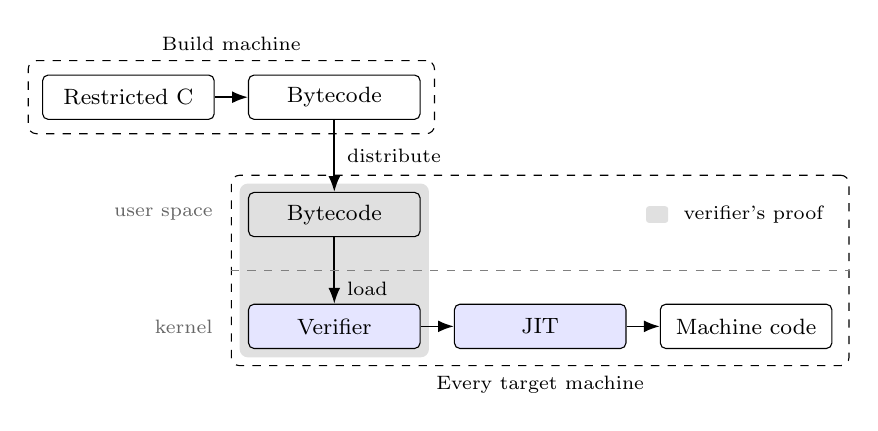
\begin{tikzpicture}[
  box/.style={draw, rounded corners=2pt, font=\footnotesize, minimum width=6.2em, minimum height=1.6em, inner sep=2pt},
  mach/.style={box, fill=blue!10},
  lbl/.style={font=\scriptsize},
  dim/.style={font=\scriptsize, text=black!60},
  arrow/.style={-Latex, semithick}
]
% 目标机器,kernel 带(下行)
\node[mach] (verif) {Verifier};
\node[mach, right=1.2em of verif] (jit) {JIT};
\node[box, right=1.2em of jit] (native) {Machine code};
% 目标机器,user space 带(中行)
\node[box, above=2.4em of verif] (byte2) {Bytecode};
% 构建机(上行)
\node[box, above=2.6em of byte2] (byte) {Bytecode};
\node[box, left=1.2em of byte] (src) {Restricted C};
% 箭头
\draw[arrow] (src) -- (byte);
\draw[arrow] (byte) -- node[lbl, right=1pt]{distribute} (byte2);
\draw[arrow] (byte2) -- node[lbl, right=1pt, pos=0.78]{load} (verif);
\draw[arrow] (verif) -- (jit);
\draw[arrow] (jit) -- (native);
% 组框
\node[draw, dashed, rounded corners=3pt, inner sep=5pt, fit=(src)(byte),
      label={[lbl]above:Build machine}] (bm) {};
\node[draw, dashed, rounded corners=3pt, inner sep=6pt, fit=(byte2)(verif)(native),
      label={[lbl]below:Every target machine}] (tm) {};
% user space 与 kernel 的分界线与带标签
\coordinate (mid) at ($(byte2.south)!0.5!(verif.north)$);
\draw[dashed, black!50, thin] (tm.west |- mid) -- (tm.east |- mid);
\node[dim, anchor=east] at ([xshift=-3pt]tm.west |- byte2.center) {user space};
\node[dim, anchor=east] at ([xshift=-3pt]tm.west |- verif.center) {kernel};
% 证明覆盖阴影(罩字节码与验证器)
\begin{scope}[on background layer]
\fill[black!12, rounded corners=3pt]
  ([xshift=-3pt,yshift=-3pt]verif.south west) rectangle ([xshift=3pt,yshift=3pt]byte2.north east);
\end{scope}
% 图例,填入 user space 带右侧空当
\node[lbl, anchor=east] (plab) at ([xshift=-6pt]tm.east |- byte2.center) {verifier's proof};
\fill[black!12, rounded corners=1pt]
  ([xshift=-10pt,yshift=-3pt]plab.west) rectangle ([xshift=-2pt,yshift=3pt]plab.west);
\end{tikzpicture}%
}
